\documentclass[12pt,letterpaper]{article}

\usepackage[margin=1in]{geometry}
\usepackage[T1]{fontenc}
\usepackage{amsmath,amssymb}
\usepackage{newtxtext,newtxmath}
\usepackage{helvet}
\usepackage{enumitem}
\usepackage{graphicx}
\usepackage{caption,booktabs}
\usepackage[hidelinks]{hyperref}
% The three required figures are included beside this source.
\graphicspath{{./}{lab3_figures/}}
\captionsetup{font=small,labelfont=bf,skip=4pt}
\renewcommand{\arraystretch}{1.15}
\setlength{\emergencystretch}{2em}

\pagestyle{empty}
\setlength{\parindent}{0pt}
\setlength{\parskip}{0pt}
\AtBeginDocument{\fontsize{12}{13.8}\selectfont}
\setlist[enumerate,1]{
  label=\arabic*.,
  leftmargin=0.25in,
  labelsep=0.08in,
  align=left,
  topsep=0pt,
  itemsep=14pt,
  parsep=6pt
}

\hypersetup{pdfauthor={Anonymous contributor},pdftitle={ECEN 474/704 - Lab 3 Prelab},pdfsubject={Anonymized laboratory prelab}}
\begin{document}

{\fontsize{11}{12.65}\selectfont
\hfill September 18, 2026\par}

{\centering
{\fontsize{14}{16.1}\selectfont\sffamily\bfseries
ECEN 474/704\par}
{\fontsize{14}{16.1}\selectfont Lab 3: Prelab\par}
{\fontsize{14}{16.1}\selectfont Anonymous contributor\par}
}

\vspace{12pt}

\begin{enumerate}

\item \textbf{Minimum transistor dimensions.}
What are the absolute minimum dimensions of a transistor? Explain your
reasoning, including the minimum contact size. Do we use this minimum
size or a slightly larger size for convenience?

\textbf{Solution.}

\textbf{(a) Minimum channel dimensions.}
For the low-voltage MOS devices used in this lab, the CMHV7SF design
manual specifies the following drawn dimensions:
\[
\boxed{L_{\min}=0.180\,\mu\mathrm{m},\qquad
W_{\min,\mathrm{channel}}=0.220\,\mu\mathrm{m}.}
\]
These are the channel dimensions, rather than the dimensions of the
entire contacted transistor layout.

\textbf{(b) Contact constraint.}
A source/drain contact (CA) is
$0.200\,\mu\mathrm{m}\times0.200\,\mu\mathrm{m}$, and the minimum
active-region (RX) enclosure is $0.100\,\mu\mathrm{m}$ on each side.
Thus the diffusion width at a contact must be at least
\[
W_{\mathrm{contact\ region}}
=0.100+0.200+0.100
=0.400\,\mu\mathrm{m}.
\]
If the source, channel, and drain use one constant-width rectangular
diffusion strip, the minimum contacted dimensions are therefore
\[
\boxed{W_{\min,\mathrm{rectangular}}=0.400\,\mu\mathrm{m},\qquad
L_{\min}=0.180\,\mu\mathrm{m}.}
\]
A $0.220\,\mu\mathrm{m}$ channel remains possible with a dogbone-shaped
diffusion region: the source/drain contact regions are widened to at
least $0.400\,\mu\mathrm{m}$, while the channel stays narrower.
The diffusion transitions must also satisfy the gate-to-RX-corner
spacing rules. A $0.200\,\mu\mathrm{m}$ contact cannot simply be placed
inside a constant-width $0.220\,\mu\mathrm{m}$ strip.

\textbf{(c) Practical choice.}
For convenient contact placement, repeated fingers, and routing, this
lab uses a slightly larger finger width:
\[
\boxed{W_f=0.500\,\mu\mathrm{m},\qquad L=0.180\,\mu\mathrm{m}.}
\]
The width is larger than the minimum contacted rectangular width,
while the channel length remains at its minimum. The
$0.500\,\mu\mathrm{m}$ width is a convenient design choice, not the
absolute minimum specified by the PDK.

{\small\textit{Rule references:} CMHV7SF Design Manual, applicable to
V1.3.1.0, Table 24, p.~67, Rules 1--2 and 10--11; Table 26, p.~77,
Rules 200 and 204. The dogbone transition is also subject to Rule 114
on p.~69.}

\newpage

\item \textbf{Common-centroid current mirror.}
Draw a common-centroid layout of a simple current mirror with equal
transistors of $L=180\,\mathrm{nm}$ and $W=12\,\mu\mathrm{m}$.
Use a finger width of $500\,\mathrm{nm}$, show the drain, source,
gate, and bulk connections, include dummy transistors, and provide
a floor plan.

\textbf{Solution.}

\textbf{(a) Finger count and floor plan.}
The number of fingers in each branch is
\[
n_f=\frac{W}{W_f}=\frac{12}{0.50}=24.
\]
There are $48$ functional fingers in total. Choose four rows of
$12$ functional fingers, with one dummy at each end of every row:
\[
\boxed{4\times12\text{ functional fingers}+8\text{ dummies}.}
\]
Let $A$ denote a reference-branch finger, $B$ an output-branch finger,
and $X$ a dummy. The floor plan is
\[
\begingroup
\setlength{\arraycolsep}{3.5pt}
\begin{array}{c|*{12}{c}|c}
X&A&B&B&A&A&B&B&A&A&B&B&A&X\\
X&B&A&A&B&B&A&A&B&B&A&A&B&X\\
X&B&A&A&B&B&A&A&B&B&A&A&B&X\\
X&A&B&B&A&A&B&B&A&A&B&B&A&X
\end{array}
\endgroup
\]
Each row contains six $A$ and six $B$ fingers, giving $24$ of each
overall. With equal finger pitch and symmetric row placement, the
two groups have the same centroid. Each functional finger has
$W_f/L=0.50/0.18\,\mu\mathrm{m}$; dummies do not contribute to the
specified effective transistor width.

\textbf{(b) Electrical connections.}
For an NMOS current mirror, use the following nets:
\[
\begin{array}{c|c|c|c|c}
\text{Finger}&D&G&S&\text{Bulk}\\ \hline
A&I_{\mathrm{IN}}&I_{\mathrm{IN}}&V_{\mathrm{SS}}&V_{\mathrm{SS}}\\
B&I_{\mathrm{OUT}}&I_{\mathrm{IN}}&V_{\mathrm{SS}}&V_{\mathrm{SS}}\\
X&\text{Adjacent }D_1\text{ or }D_2&V_{\mathrm{SS}}&V_{\mathrm{SS}}&V_{\mathrm{SS}}
\end{array}
\]
The reference branch is diode-connected:
$G=D_1=I_{\mathrm{IN}}$. All functional gates share this node, while
$D_2=I_{\mathrm{OUT}}$. Each dummy has $V_{GS}=0$ and its gate is
isolated from the functional gate bus. Substrate taps connect the
bulk to $V_{\mathrm{SS}}$.

\begin{quote}
\begin{minipage}{\linewidth}
\centering
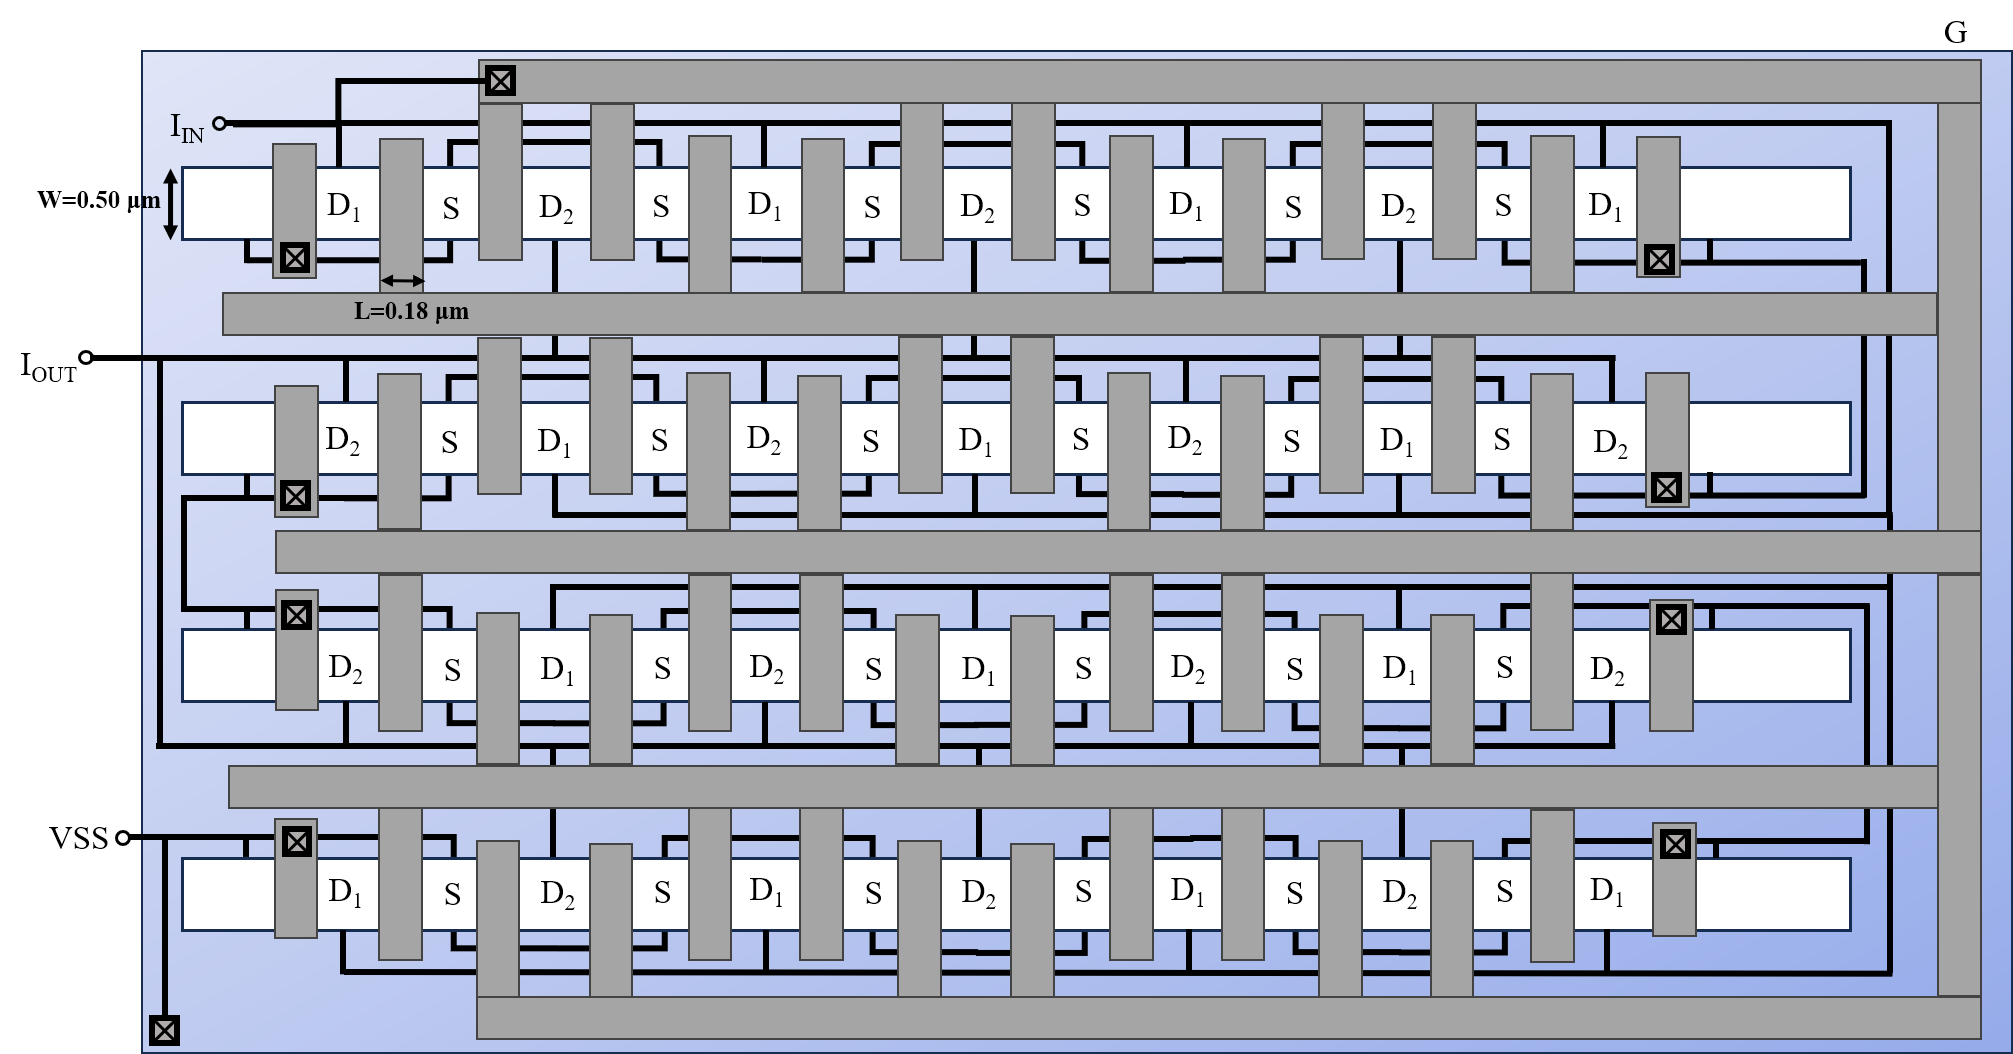
\includegraphics[width=\linewidth,height=0.40\textheight,keepaspectratio]{current_source.png}
\captionof{figure}{Common-centroid current-mirror layout with four rows,
twelve functional fingers per row, and eight edge dummies.}
\label{fig:lab3-current-mirror}
\end{minipage}
\end{quote}

\textbf{(c) Matching considerations.}
Use equal finger dimensions and regular spacing, share diffusion
where appropriate, and balance the drain routing, contact counts,
and parasitic loading between the branches. The outer two rows and
inner two rows exchange $A$ and $B$, balancing the drain regions at
the row ends. Common-centroid placement suppresses first-order
spatial-gradient mismatch; it does not eliminate random mismatch.

\newpage

\item \textbf{Common-centroid MOM capacitor array.}
Draw a common-centroid MOM capacitor array with
$C_1:C_2=1:1.4$, using eight unit capacitors
($I_1=I_2=4$) and one non-unit capacitor. Each unit measures
$10.56\,\mu\mathrm{m}\times10.56\,\mu\mathrm{m}$.
Determine the non-unit dimensions, show the interconnections,
and include dummy capacitors and suitable matching techniques.

\textbf{Solution.}

\textbf{(a) Required non-unit capacitance.}
Let $C_u$ be the unit capacitance and $C_{\mathrm{nu}}=NC_u$.
Then
\[
C_1=4C_u,\qquad C_2=(4+N)C_u,\qquad
\frac{4}{4+N}=\frac{1}{1.4}.
\]
Therefore,
\[
\boxed{N=1.6,\qquad C_{\mathrm{nu}}=1.6C_u,\qquad C_2=5.6C_u.}
\]

\textbf{(b) Non-unit capacitor dimensions.}\par
Using $L_0=10.56\,\mu\mathrm{m}$ and the lab manual's
area/perimeter matching formulas,
\begin{align*}
L_{\mathrm{nu}}
&=L_0\left[N+\sqrt{N(N-1)}\right]\\
&=10.56\left[1.6+\sqrt{1.6(0.6)}\right]
=27.24264467\,\mu\mathrm{m},\\
W_{\mathrm{nu}}
&=\frac{NL_0^2}{L_{\mathrm{nu}}}
=\frac{1.6(10.56)^2}{27.24264467}
=6.54935533\,\mu\mathrm{m}.
\end{align*}
Thus,
\[
\boxed{W_{\mathrm{nu}}\times L_{\mathrm{nu}}
\simeq6.549\,\mu\mathrm{m}\times27.243\,\mu\mathrm{m}.}
\]
The area and perimeter scale by the same factor:
\begin{align*}
A_u&=111.5136\,\mu\mathrm{m}^2,
&P_u&=42.24\,\mu\mathrm{m},\\
A_{\mathrm{nu}}&=178.42176\,\mu\mathrm{m}^2=1.6A_u,
&P_{\mathrm{nu}}&=67.584\,\mu\mathrm{m}=1.6P_u.
\end{align*}
Consequently, $P_{\mathrm{nu}}/A_{\mathrm{nu}}=P_u/A_u$.
These are the nominal dimensions from the lab's matching construction;
the implemented MOM capacitance also depends on the PDK model and
available geometry increments.

\textbf{(c) Common-centroid floor plan.}
Place the four $A$ units of $C_1$ at the corners of the inner array,
the four $B$ units of $C_2$ at the side centers, and
$C_{\mathrm{nu}}$ at the center. Surround the array with unit-size
dummies $X$:
\[
\begin{array}{ccccc}
X&X&X&X&X\\
X&A_1&B_1&A_2&X\\
X&B_2&C_{\mathrm{nu}}&B_3&X\\
X&A_3&B_4&A_4&X\\
X&X&X&X&X
\end{array}
\]
This gives four $A$ units, four $B$ units, one non-unit capacitor,
and sixteen dummies. The table denotes placement, not equal-size
physical cells: $C_{\mathrm{nu}}$ is a long rectangle, so the spacing
must accommodate it symmetrically. Both unit groups have their
centroids at the center, and adding the centered $C_{\mathrm{nu}}$
preserves the capacitance-weighted centroid of $C_2$.

\textbf{(d) Interconnections and matching.}
Connect $A_1$--$A_4$ in parallel and connect $B_1$--$B_4$ and $C_{\mathrm{nu}}$ in parallel.
In particular, $C_{\mathrm{nu}}$ belongs only to $C_2$.
All backplate terminals connect to $V_{\mathrm{SS}}$.

Use identical orientation and local routing for the unit capacitors,
multiple contacts where appropriate, and balanced routing parasitics.
Following Fig.~3-10 of
the lab manual, short the two signal terminals of each dummy together
as an individual floating node; its backplate remains connected to
$V_{\mathrm{SS}}$.

\begin{quote}
\begin{minipage}{\linewidth}
\centering
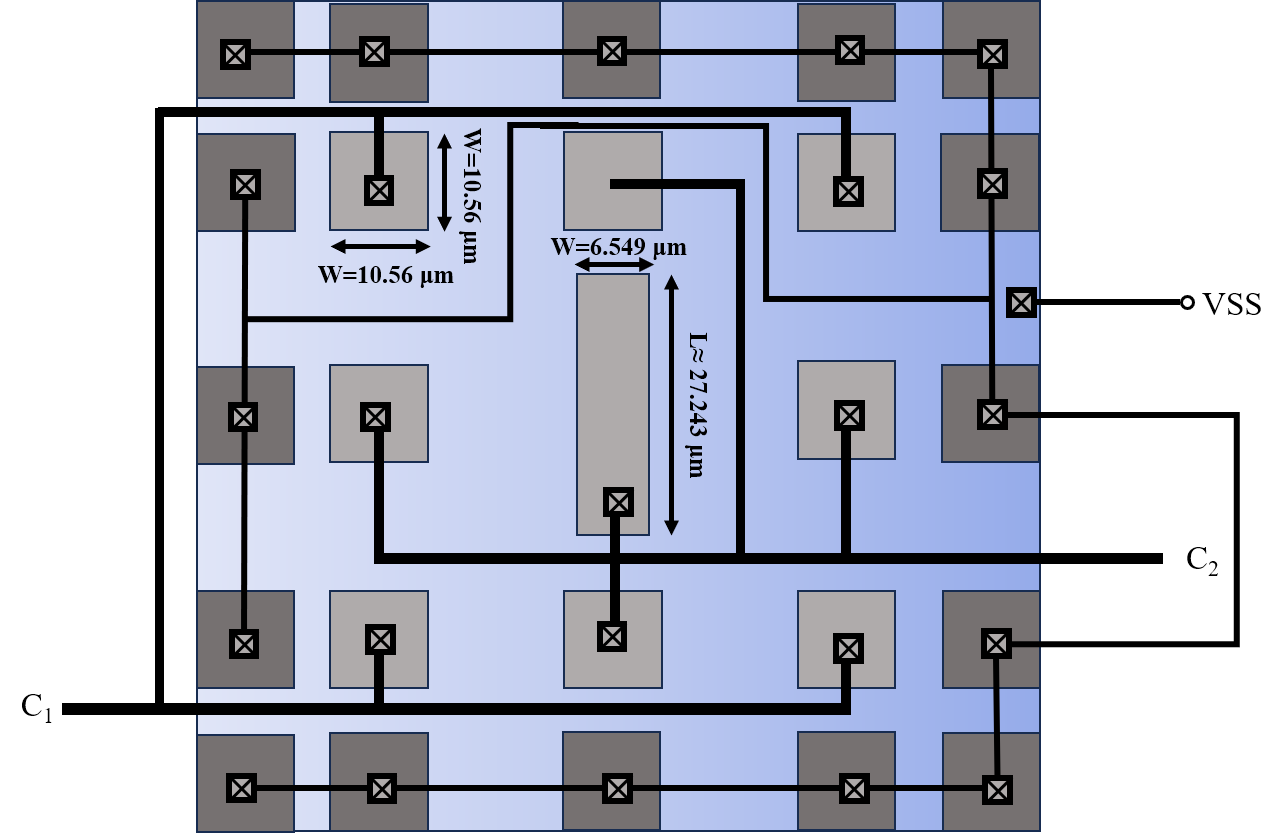
\includegraphics[width=\linewidth,height=0.48\textheight,keepaspectratio]{capacitor.png}
\captionof{figure}{Common-centroid MOM capacitor array.
The four $C_1$ units are connected in parallel; the four $C_2$ units
and the centered non-unit capacitor are connected in parallel.}
\label{fig:lab3-capacitor}
\end{minipage}
\end{quote}

\newpage

\item \textbf{Interdigitized matched polysilicon resistors.}
Draw two matched \texttt{oprppresx} resistors of
$15\,\mathrm{k}\Omega$ each, using four series segments per resistor.
Account for contact resistance, determine the segment length and width,
and use an interdigitized layout. The combined component area of the
two resistors must be between $30$ and $80\,\mu\mathrm{m}^2$.

\textbf{Solution.}

\textbf{(a) Segment dimensions including contact resistance.}
Each of the four series segments must have nominal resistance
\[
R_{\mathrm{seg}}=\frac{15}{4}=3.75\,\mathrm{k}\Omega.
\]
From Table 3-1 of the lab manual,
\[
R_s=0.165\,\mathrm{k}\Omega/\square,\qquad
R_{\mathrm{con}}=0.015\,\mathrm{k}\Omega\cdot\mu\mathrm{m}.
\]
The nominal resistance of each contacted segment is
\[
R_{\mathrm{seg}}=R_s\frac{L}{W}+\frac{2R_{\mathrm{con}}}{W}.
\]
Choose $W=0.50\,\mu\mathrm{m}$. Measuring $L$ in
$\mu\mathrm{m}$ and resistance in $\mathrm{k}\Omega$ gives
\[
3.75=0.165\frac{L}{0.50}+\frac{2(0.015)}{0.50}
=0.33L+0.06.
\]
Therefore,
\[
\boxed{L=11.1818\,\mu\mathrm{m},\qquad W=0.50\,\mu\mathrm{m}.}
\]
Each segment contributes $3.69\,\mathrm{k}\Omega$ from its body and
$0.06\,\mathrm{k}\Omega$ from its two contacts. Hence
\[
\boxed{R_1=R_2=4(3.69+0.06)=15.00\,\mathrm{k}\Omega.}
\]
The length $L$ is the effective resistor-body length defined by the
OP mask, rather than the full strip length including the contact ends.

\textbf{(b) Area check.}
The combined body area of the eight functional segments is
\[
A_{\mathrm{active}}=8WL
=8(0.50)(11.1818)
\simeq\boxed{44.73\,\mu\mathrm{m}^2},
\]
which lies between $30$ and $80\,\mu\mathrm{m}^2$.
Including two identical dummy bodies gives approximately
$55.91\,\mu\mathrm{m}^2$. The overall layout footprint is larger
because contacts, routing, and spacing require additional area.

\textbf{(c) Placement and series connections.}
Place ten parallel strips with equal orientation and spacing:
\[
\begin{array}{cccccccccc}
X&A_1&B_1&A_2&B_2&A_3&B_3&A_4&B_4&X.
\end{array}
\]
The two groups are spatially interdigitized and electrically connected as
\begin{align*}
\mathrm{R1}&\longrightarrow A_1\longrightarrow A_2
\longrightarrow A_3\longrightarrow A_4\longrightarrow\mathrm{R1},\\
\mathrm{R2}&\longrightarrow B_1\longrightarrow B_2
\longrightarrow B_3\longrightarrow B_4\longrightarrow\mathrm{R2}.
\end{align*}
For a serpentine connection, join the bottom ends of segments 1 and 2,
the top ends of segments 2 and 3, and the bottom ends of segments 3
and 4 within each group. The top ends of segments 1 and 4 are the
external terminals. This is an interdigitized arrangement, as requested;
the single-row $ABABABAB$ pattern is not common-centroid.

\begin{quote}
\begin{minipage}{\linewidth}
\centering
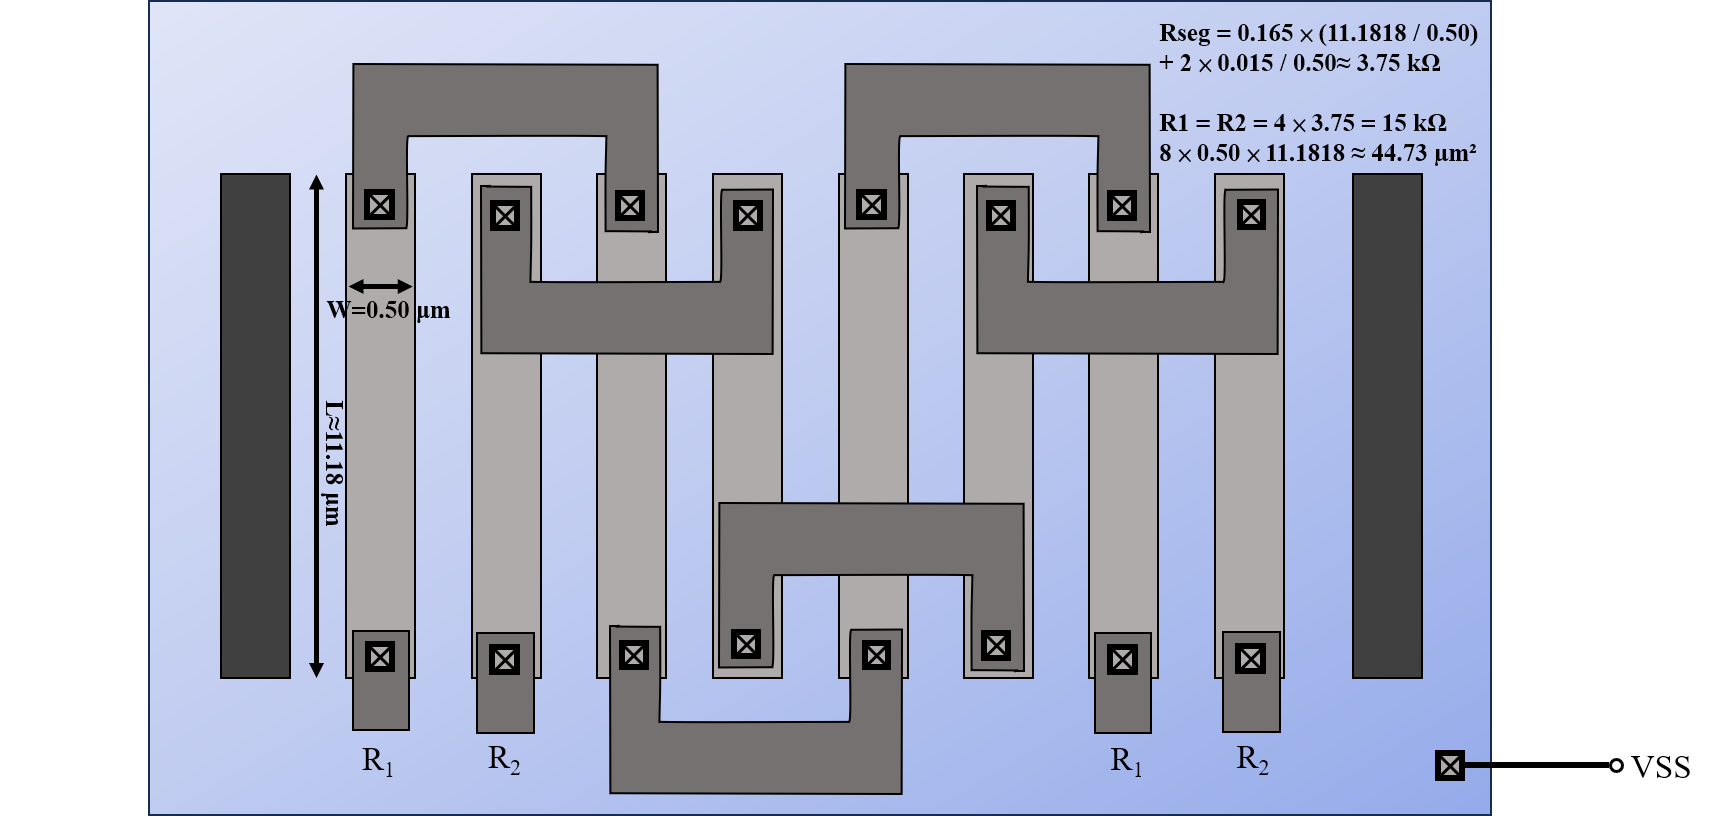
\includegraphics[width=\linewidth,height=\textheight,keepaspectratio]{resistor.png}
\captionof{figure}{Interdigitized matched resistor pair with four
series segments per resistor and one dummy strip at each outer edge.}
\label{fig:lab3-resistor}
\end{minipage}
\end{quote}

\textbf{(d) Matching and substrate connections.}
Keep segment geometry, contact counts, routing lengths, and the
lengths of metal overlapping the resistor bodies balanced between
the two groups. Where separate nets cross, use different metal layers
without an interconnecting via, while balancing the layer usage and
via counts between the groups.

Following Fig.~3-14 of the lab manual, leave each dummy's two signal
terminals individually floating. All resistor backplates, including those of the dummies, connect to $V_{\mathrm{SS}}$.

\end{enumerate}

\end{document}
